
%%%%%%%%%%%%%%%%%%%%%%% file typeinst.tex %%%%%%%%%%%%%%%%%%%%%%%%%
%
% This is the LaTeX source for the instructions to authors using
% the LaTeX document class 'llncs.cls' for contributions to
% the Lecture Notes in Computer Sciences series.
% http://www.springer.com/lncs       Springer Heidelberg 2006/05/04
%
% It may be used as a template for your own input - copy it
% to a new file with a new name and use it as the basis
% for your article.
%
% NB: the document class 'llncs' has its own and detailed documentation, see
% ftp://ftp.springer.de/data/pubftp/pub/tex/latex/llncs/latex2e/llncsdoc.pdf
%
%%%%%%%%%%%%%%%%%%%%%%%%%%%%%%%%%%%%%%%%%%%%%%%%%%%%%%%%%%%%%%%%%%%


\documentclass[runningheads,a4paper]{llncs}

\usepackage{amssymb}
\setcounter{tocdepth}{3}
\usepackage{graphicx}
\usepackage{epstopdf}
\usepackage{subfig}
\usepackage{array}

\graphicspath{{images/}}

\usepackage{url}
\urldef{\mailsa}\path|ary506@york.ac.uk|
\newcommand{\keywords}[1]{\par\addvspace\baselineskip
\noindent\keywordname\enspace\ignorespaces#1}

\begin{document}

\mainmatter  % start of an individual contribution

% first the title is needed
\title{Gamification of Software Modelling Learning}

% a short form should be given in case it is too long for the running head
\titlerunning{Gamification of Software Modelling Learning}

% the name(s) of the author(s) follow(s) next
%
% NB: Chinese authors should write their first names(s) in front of
% their surnames. This ensures that the names appear correctly in
% the running heads and the author index.
%
\author{Alfa Yohannis}
%
\authorrunning{Gamification of Software Modelling Learning}
% (feature abused for this document to repeat the title also on left hand pages)

% the affiliations are given next; don't give your e-mail address
% unless you accept that it will be published
\institute{Department of Computer Science, University of York, York, United Kingdom\\
\mailsa\\}

%
% NB: a more complex sample for affiliations and the mapping to the
% corresponding authors can be found in the file "llncs.dem"
% (search for the string "\mainmatter" where a contribution starts).
% "llncs.dem" accompanies the document class "llncs.cls".
%

\toctitle{Lecture Notes in Computer Science}
\tocauthor{Gamification of Software Modelling Learning}
\maketitle


\begin{abstract}
The abstract should summarize the contents of the paper and should
contain at least 70 and at most 150 words. It should be written using the
\emph{abstract} environment.
\keywords{software modelling, gamification, learning}
\end{abstract}


\section{Introduction}
Software modelling is commonly perceived as an difficult subject since it requires a great deal of abstractions \cite{Borstler2012}. However, this subject has a fundamental and crucial role in software engineering. Failure to master this subject will affect the student’s abstraction capability in analysing and designing a real-world software. Less proficiency in software modelling will likely cause software engineering students facing difficulties completing their degrees, as most of the software engineering related subjects have a sense of intrinsic abstraction problems \cite{Kramer2007}. Their perception of software modelling will affect their attitude towards software engineering today and their career paths in the future.

For new software engineering students, software modelling is commonly perceived as subjects that are difficult to learn. Software, by its nature, is abstract and complex that demand loads of abstraction to model it. This problem is similar to problems in mathematics where much of the concepts can only be accessed through symbolical representations \cite{Duval2006}. Abstraction also means requiring the students to perform information hiding, generalization, approximation or reformulation, leaving out the irrelevant aspects but keeping the relevant ones, or separation from the concrete reality \cite{Saitta2013}. In order to overcome these challenges, we need to put more efforts on delivering software modelling in a more concrete and motivating presentation which can engage and ease students to learn it.

On the other hand, the use of games or game elements for serious purposes other than leisure has drawn lots of attentions. Gamification \cite{deterding2011game} and Serious Games \cite{Michael2005} have been viewed as solutions to solve motivational problems that emerge when users engage in  boring, irrelevant, difficult activities, e.g. learning sorting algorithms \cite{Yohannis2015} or C-programming \cite{Ibanez2014}.

Therefore, the purpose of this research is to investigate and develop a gamification design framework that systematically and semi-automatically drive gamification design to produce better-design software modelling games. More precisely, this research aims to answer the following research questions that are derived from the purpose of this research:
\begin{enumerate}
\item Which processes, aspects, principles, or components of software modelling and their teaching and learning practices that are essential to take into account?
\item What types of game elements and their roles that can deliver software modelling at best? 
\item What kind of framework that orchestrates, design the interaction between, software modelling and game elements to produce a better software modelling gamification?
\item To what extend gamification of software modelling better engage, motivate, and improve learners’ performances?
\end{enumerate}

\section{Related Works}

Several approaches have been conducted to bring software modelling into a more concrete presentation that can be easily understood by learners, ranging from didactic learning \cite{moisan2009teaching}, modeling tools utilization \cite{Akayama2013}, alternative communication channels and the use of modelling language \cite{Brandsteidl2011}, immersive visual modelling through virtual environment \cite{neubauer2003immersive}, software design studio \cite{Whittle2014}, project-based approach \cite{Szmurlo2007}, to code generation investigation \cite{schmidt2014teaching}.

However, most of the approaches have weaknesses in motivating learners to engage continuously, frequently, and actively to learn software modelling, which is the important aspect to impact greatly on learning \cite{Naps2005}. This condition then elevates game as one approach, a.k.a. game-based learning, to learn or teach software modelling. This approach provides students a new way of learning software modelling, which is not only interactive but also engaging enough to keep them learning continuously. 

The use of game elements for a purpose other than leisure is called gamification \cite{deterding2011game} or  the process of transforming a less gameful entity into a more gameful one \cite{Werbach2014} \cite{Kapp2012} \cite{Yohannis2014}. Regardless gamification design is still an ongoing challenge \cite{Deterding2013}, it is an opportunity for research that up today there is still no gamification design framework that particularly address how to guide the design of software modelling gamification; a framework that guides how to integrate game specific domain into software modelling. Therefore, this research aims to develop a gamification design framework of software modelling.

Most of the gamification studies available are dominantly relates to software engineering in a larger context or other aspects of software engineering, such as software implementation and project management, rather than software modelling in particular \cite{Pedreira2015}. After the literature exploration, only four works have been identified applied gamification for software modelling. In their work, Groenewegen et al. \cite{Groenewegen2010} implemented cards, explorable board-game, and rules to help the audience to learn and validate enterprise architecture models. The gamification works by facilitating the audience to explore a model step by step, element by element according to the given rules similar to a map board game. This method provides a progressive user experience helping the audience to understand the model through provoking curiosity so they can give argument whether the model is valid or not based on their existing knowledge. However, the pedagogical aspect was not discussed explicitly  in their publication and the evaluation was limited to a very small number of respondents. 

Stikkolorum et al. \cite{Stikkolorum2014} implemented puzzle game, levels, visual and audio feedbacks, progress indicator, level unlocking, choice of path, multiple solutions, and scoring to teach cohesion, coupling, information hiding, and modularity in software design. The outcome is the audience started to talk about classes, methods, and associations instead of boxes, blocks, and lines, indication of unconscious learning. Nevertheless, the pedagogical aspect was not discussed deeply and the evaluation is limited to a very small respondents using the 'think aloud' method. Ionita et al. \cite{Ionita2015} developed a socio-technical modelling language (TREsPASS) and map them toward tangible representation. The tangible representations will increase the familiarity and understandability of the model, therefore increase awareness and involvement. For the game  elements, they used familiar and tangible representation---such as Lego characters and board-game metaphor---and rules to improve learnability and participation. Nonetheless, their work is specific to domain modelling in information security, not for learning software modelling in general. Richardsen \cite{Richardsen2014} utilised UML activity diagram to control the behaviour of a game. The purpose of his research is to support the audience learning activity diagram in the context of Reactive Block tools and comparing the learning outcomes between the traditional interactive tutorial and the game-like one. Even though the game-like tutorial is more engaging, there is no significant difference between the the game-like tutorial and the traditional one. Moreover, the number of respondents for evaluation was very limited and no pedagogical aspect was discussed.

\section{Research Methods}
Since the output of this work is design artefacts, we decided to utilise the Design Science Research Methodology (DSRM) \cite{peffers2007design} as our umbrella methodology. DSRM is selected because it provides a comprehensive high-level conceptual framework how to undergo a full-cycle research process. It also provides six-activity guidelines for understanding, developing, executing, and evaluating design artifacts. The six activities are (1) problem identification and motivation activity, (2) define objectives for a solution activity, (3) define objectives for a solution activity, (4) design and development activity, (5) demonstration and evaluation activities, and (6) communication. 

The high-level characteristic means that we can employ other research methods as the sub methods in each activity. For examples, we employ interviews, literature reviews, and discussion with experts as our methods in problem identification and motivation activity as well as utilise Deterding's lens of intrinsic skill atoms \cite{deterding2015lens} to produce a gameful design in the design and development activity. We use the activities of DSRM as the guidelines to report this research's in-progress accomplishment in the following sections.
 
\section{Analysis}
Problem Identification and Motivation.
Solution and Objective Definition.

\section{Design}
In this section, I describe the design applied on the artefact. The design process are driven by the Design Lenses and Skill Atoms \cite{deterding2015lens}. The mechanics, interface, model editor, model validation, and evaluation are also briefly presented in this section.

\subsection{Gamification Design}
In order to deliver a gameful experience while playing with the artefact, game elements have to embedded into the artefact's design. Thus, Design Lenses and Skill Atoms are utilised to determine the required game elements and game mechanics. Tables \ref{Table001} and Table \ref{Table002} show the Design Lenses and Skill Atoms applied in the gamification design.

\begin{table}[htb]
\caption{Design lenses (game elements) applied in the gamification design.}\label{Table001}
\begin{center}
    \begin{tabular}{ | p{3.2cm} | p {8.8cm} | }
    \hline
	\textbf{Lenses} & \textbf{Elements}\\    
    \hline
    Challenges & Onboarding, scaffolded challenge, varied challenge \\    
    \hline
    Goals and Motivation & interim goals, intrinsic rewards, templates\\
    \hline
	Actions and Object & bite sized actions, limited choices, microflow, underdetermination, sensual \\
    \hline
    Feedbacks & Immediate, juicy, acti onable, appeal to motives, glanceable, varied, graspable progress\\
    \hline
    \end{tabular}
\end{center}
\end{table}


\begin{table}[htb]
\caption{Skill Atoms applied in the gamification design.}\label{Table002}
\begin{center}
    \begin{tabular}{ | p{3.2cm} | p {8.8cm} | }
    \hline
	\textbf{Atoms} & \textbf{Description}\\    
    \hline
    Motivation & Master the modelling (solve problem, able to construct model) \\    
    \hline
    Goals & Create models that satisfy requirements \\
    \hline
	Actions and Objects & Construct model using diagrams, elements of a diagram, keywords, hints \\
    \hline
    Challenges & Satisfy requirements, meet objectives\\
    \hline
	Rules & Inherent rules in every model diagram, constraints, objectives\\
	\hline
	Feedbacks & completed objectives, model metrics, and motivating words\\
	\hline
    \end{tabular}
\end{center}
\end{table}


\begin{figure}[htb]
\centering
\subfloat[Level Selection]{\frame{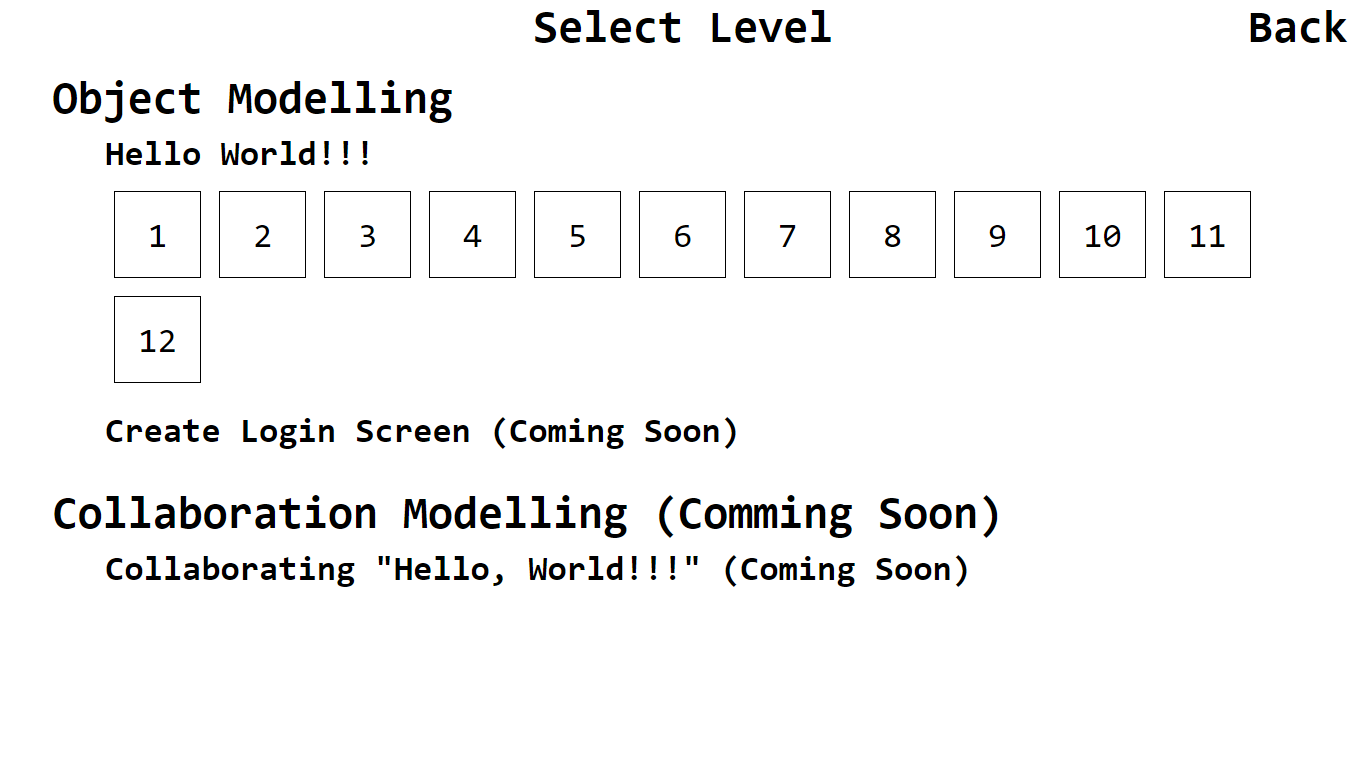
\includegraphics[height=3.5cm]{levels}}}
\hspace*{\fill}
\subfloat[Positive Reinforcement]{\frame{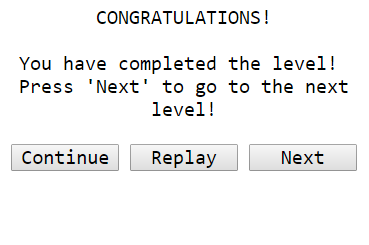
\includegraphics[height=3.5cm]{positive}}}
\caption{Game and learning elements embedded into the artifact.}
\end{figure}

\begin{figure}[htb]
\centering
\frame{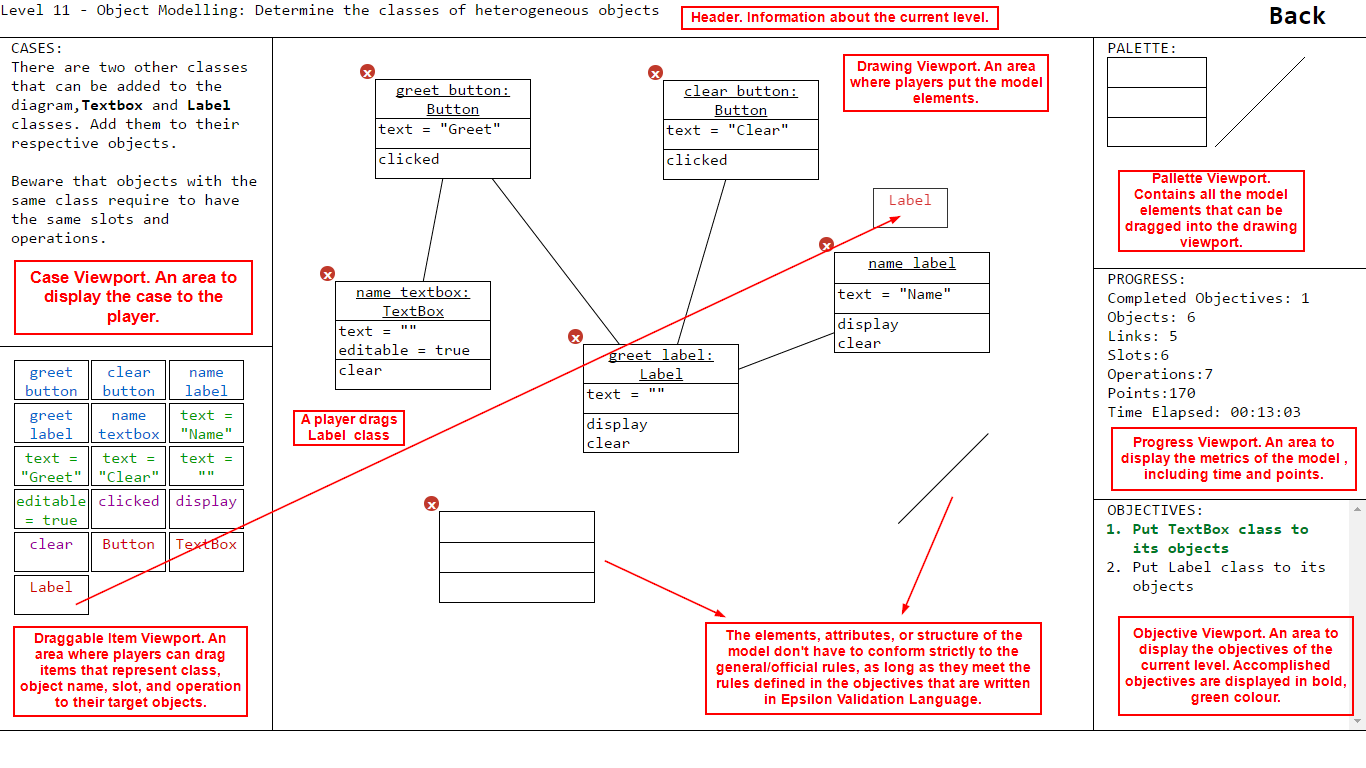
\includegraphics[width=\textwidth]{game-annotated}}
\caption{The game's display.}
\end{figure}

\subsection{Architecture}

\subsection{Model Validation}

\subsection{Modelling Editor}

\begin{figure}[htb]
\centering
\frame{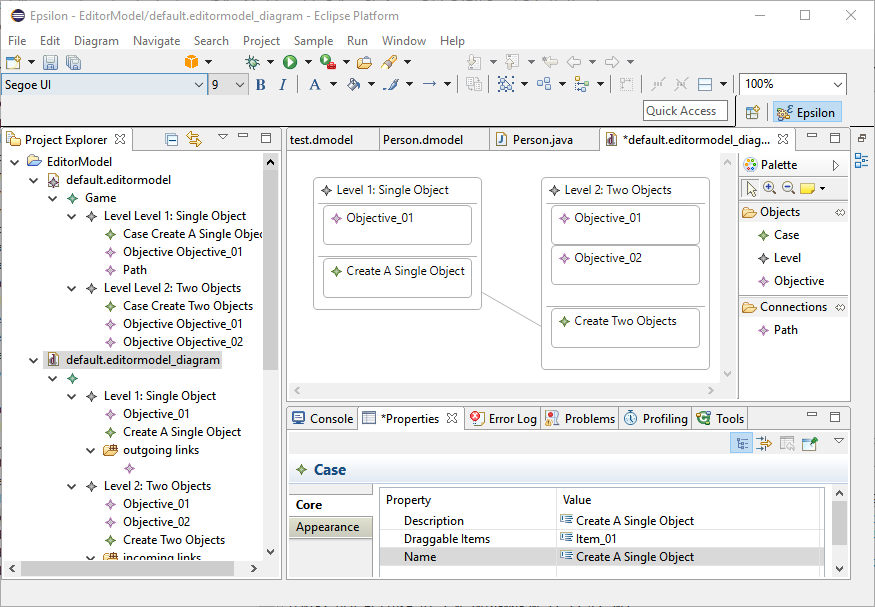
\includegraphics[width=\textwidth]{editor}}
\caption{Game editor to automatically generate the game.}
\end{figure}

\section{Evaluation}

\section{Conclusion}
 

\subsubsection*{Acknowledgments.} We would like to thank our respondents that participated in our preliminary interview. This research is supported by \emph{Lembaga Pengelola Dana Pendidikan Indonesia} (Indonesia Endowment Fund for Education). 

\bibliography{references} 
\bibliographystyle{ieeetr}

\end{document}

